
\documentclass[]{BasiliskReportMemo}

\usepackage{cite}
\usepackage{AVS}
\usepackage{float} %use [H] to keep tables where you put them
\usepackage{array} %easy control of text in tables
\usepackage{graphicx}
\bibliographystyle{plain}


\newcommand{\submiterInstitute}{Autonomous Vehicle Simulation (AVS) Laboratory,\\ University of Colorado}


\newcommand{\ModuleName}{inertial3D}
\newcommand{\subject}{Guidance Module to Perform an Inertially Fixed Pointing}
\newcommand{\status}{Version 1.2}
\newcommand{\preparer}{M. Cols}
\newcommand{\summary}{Generate the reference attitude trajectory for a general 3D inertial pointing.  A corrected body frame will align with the desired reference frame.     }


\begin{document}


\makeCover


%
%	enter the revision documentation here
%	to add more lines, copy the table entry and the \hline, and paste after the current entry.
%
\pagestyle{empty}
{\renewcommand{\arraystretch}{2}
\noindent
\begin{longtable*}{|p{0.5in}|p{4.5in}|p{1.14in}|}
\hline
{\bfseries Rev}: & {\bfseries Change Description} & {\bfseries By} \\
\hline
Draft & initial copy & M. Cols \\
1.1 & Updated template to BSK from AVS & D. Burder \\
1.2 & Added test result discussion and user guide section & H. Schaub  \\
\hline

\end{longtable*}
}

\newpage
\setcounter{page}{1}
\pagestyle{fancy}

\tableofcontents %Autogenerate the table of contents
~\\ \hrule ~\\ %Makes the line under table of contents


% !TEX root = ./Basilisk-Inertial3D-2016-01-15.tex


\section{Model Description}

This technical note discusses the guidance mathematics to compute a reference frame $\mathcal{R}$ that is aligned the with an inertially fixed  frame  $\mathcal{R}_0$, as shown in Figure~\ref{fig:Fig1}.
\begin{figure}[htb!]
	\centerline{
	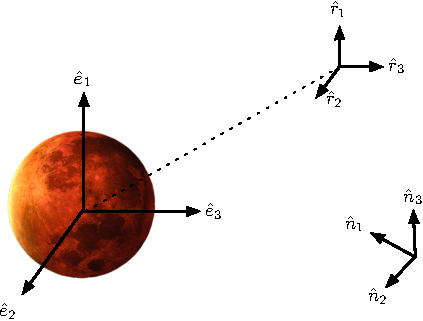
\includegraphics{Figures/Fig3}
	}
	\caption{Illustration of the input inertially fixed frame $\mathcal{R}_{0}:\{ \hat e_{1}, \hat e_{2}, \hat e_{3} \}$, the generated reference frame $\mathcal{R}: \{ \hat r_{1}, \hat r_{2}, \hat r_{3}\}$ and the inertial frame $\mathcal{N}:\{ \hat{\bm n}_{1}, \hat{\bm n}_{2}, \hat{\bm n}_{3} \}$}
	\label{fig:Fig1}
\end{figure}

\subsection{Reference Frame Generation}
The modules requires the desired reference orientation in terms of the MRP set $\bm{\sigma}_{R_{0}N}$. This input is only set once and does not have to be changed.
Let us designate $\mathcal{R}$ as the output generated reference frame. Since the fixed-pointing is inertial:
\begin{equation}
	\bm{\sigma}_{RN} = \bm{\sigma}_{R_{0}N}
\end{equation}
\begin{equation}
	\bm{\omega}_{RN} = \dot{\bm{\omega}}_{RN} = 0
\end{equation}

\subsection{Module Input and Output}
Table ~\ref{tab:inputTable} shows the input Configuration Data of the module Inertial 3D Point.
\begin{table}[h!]
	\centering
	\caption{Input Configuration Data}
	\begin{tabular}{|l|l|l|p{3in}|}
		\hline
		Name & Type & Length & Description \\
		\hline
		$\sigma_{R_0/N}$ & double [ ] & 3 & 
		MRP attitude set of the desired reference frame with respect to the inertial frame . \\ \hline
	\end{tabular}
	\label{tab:inputTable}
\end{table}


Table ~\ref{tab:outputTable} shows the Attitude Reference output message of the module Inertial 3D Point.
\begin{table}[h!]
	\centering
	\caption{Output Attitude Reference Message}
	\begin{tabular}{|l|l|l|p{3in}|}
		\hline
		Name & Type & Length & Description \\ \hline
		$\sigma_{R/N}$ & double [ ] & 3 & 
		MRP attitude set of the reference frame with respect to the inertial frame. \\ \hline
		$\leftexp{N} \omega_{R/N}$ & double [ ] & 3 & 
		Angular rate vector of the reference frame with respect to the inertial expressed in inertial frame components. \\ \hline
		$\leftexp{N} {\dot{\omega}_{R/N}}$ & double [ ] & 3 & 
		Angular acceleration vector of the reference frame with respect to the inertial expressed in inertial frame components. \\ \hline
	\end{tabular}
	\label{tab:outputTable}
\end{table}\\


 %This section includes mathematical models, code description, etc.

% !TEX root = ./Basilisk-thrFiringSchmitt-2019-03-29.tex



\section{Module Functions}
\begin{itemize}
	\item \textbf{Read in thruster configuration message}: This is used to determine the number of installed thrusters and what the maximum force is for each.
	\item \textbf{Convert thruster force requested into an on-time request}: Knowing how strong the thruster is, the on-time is scaled such that the effectively applied force is equal to the requested force.
\end{itemize}

\section{Module Assumptions and Limitations}
The module assumes that the incoming forces $F_{i}$ can be both positive or negative, depending if an on- or off-pulsing mode is being implemented.  The particular mode is set through {\tt baseThrustState}.   %This includes a concise list of what the module does. It also includes model assumptions and limitations

% !TEX root = ./Basilisk-sunSafePoint-20180427.tex

\section{Test Description and Success Criteria}
The mathematics in this module are straight forward and can be tested in a series of input and output evaluation tests.


\subsection{Check 1}
Here a check is performed where the sun vector measurement $\bm s$ has a non-zero length and is not aligned with $\hat{\bm s}_{c}$.  

\subsection{Check 2}
The sun direction vector $\bm s$ is given a norm value that is less than {\tt minUnitMag}.  In this case the attitude tracking $\bm\sigma_{B/R}$ should be set to zero.  Further, the body rate errors are now evaluated relative to a fixed $\bm\omega_{R/N}$ vector.  

\subsection{Check 3}
The sun direction vector $\bm s$ aligned with $\hat{\bm s}_{c}$.  In this case the attitude tracking $\bm\sigma_{B/R}$ should be set to zero.  Further, the body rate errors are simply the inertial body angular rates.  

\subsection{Check 4}
The sun direction vector $\bm s \approx -\hat{\bm s}_{c}$.  In this case the attitude tracking $\bm\sigma_{B/R}$ should be set to $\hat{\bm e}_{180}$.  Further, the body rate errors are simply the inertial body angular rates.  

\subsection{Check 4}
The sun direction vector $\bm s \approx -\hat{\bm s}_{c}$, but $\hat{\bm s}_{c} = \hat{\bm b}_{1}$.  In this case the attitude tracking $\bm\sigma_{B/R}$ should be set to $\hat{\bm e}_{180}$ that is evaluated with the cross product with $\hat{\bm b}_{2}$.  Further, the body rate errors are simply the inertial body angular rates.  


\section{Test Parameters}
The unit test verify that the module output guidance message vectors match expected values.
\begin{table}[htbp]
	\caption{Error tolerance for each test.}
	\label{tab:errortol}
	\centering \fontsize{10}{10}\selectfont
	\begin{tabular}{ c | c } % Column formatting, 
		\hline\hline
		\textbf{Output Value Tested}  & \textbf{Tolerated Error}  \\ 
		\hline
		$\bm\sigma_{B/R}$        & \input{AutoTex/toleranceValue}	   \\ 
		$\bm\omega_{B/R}$        & \input{AutoTex/toleranceValue}\\ 
		$\bm\omega_{R/N}$        & \input{AutoTex/toleranceValue} \\ 
		$\dot{\bm\omega}_{R/N}$        & \input{AutoTex/toleranceValue}  \\ 
		\hline\hline
	\end{tabular}
\end{table}

The nominal module test input values are $\hat{\bm s}_{c} = (0,0,1)$, $\bm s = (1,0,0)$ and $\leftexp{B}{\bm\omega}_{B/N} = (0.01, 0.50, -0.20)$ rad/sec.  The nominal body-fixed search rate is set to $\leftexp{B}{\bm\omega}_{R/N} = (0.0, 0.0, 0.1)$ rad/sec.  This rate is only used if no sun direction vector is available.  The small angle is set to $\epsilon$ = 0.01 degrees.  



\section{Test Results}

All of the tests passed:
\begin{table}[H]
	\caption{Test results}
	\label{tab:results}
	\centering \fontsize{10}{10}\selectfont
	\begin{tabular}{c | c  } % Column formatting, 
		\hline\hline
		\textbf{Check} 						  		&\textbf{Pass/Fail} \\ 
		\hline
	   1	   			& \input{AutoTex/passFail1} \\ 
	   2	   			& \input{AutoTex/passFail2} \\ 
	   3	   			& \input{AutoTex/passFail3} \\ 
	   4	   			& \input{AutoTex/passFail4} \\ 
	   5	   			& \input{AutoTex/passFail5} \\ 
	   \hline\hline
	\end{tabular}
\end{table}



 % This includes test description, test parameters, and test results

\section{User Guide}
For the best examples of the using the Gauss Markov utility, please see the IMU unit test and .cpp files. For other examples, see the simple navigation unit and coarse sun sensor. % Contains a discussion of how to setup and configure  the BSK module



\bibliographystyle{unsrt}
\bibliography{references}

\end{document}
